
\section{Advances on cartographic\\ document formats}\label{advances-on-cartographic-document-format}
\label{advances}

The focus of this work is the definition of a novel format of cartographic
documents along with the software ecosystem rooted on it. A simple but
effective algorithm to find indoor valid routes is also provided. HIJSON
(Hierarchical Indoor JSON) is the name chosen for the new document format; 
it the accompanying software framework, aim to realize a
mapping of real indoor spaces with a virtual interactive web environment.
HIJSON is based upon ideas and design principles collected from previous
formats and identifies four critical improvements with respect to them: it
exposes a \emph{hierarchical structure}, uses \emph{metric local coordinate
system}, may import \emph{external geometric models} and accepts \emph{semantic
extensions}. 
% Furthermore, geometrical  and topological data are conveniently imported and represented via LAR, an advanced  representation scheme, allowing to deal with \emph{hyperlinked geometric models}.

\subsection{Hierarchical structure}\label{hierarchical-structure}

The HIJSON format allows for hierarchical description of indoor spaces. The
introduction of a hierarchical structure establishes a parent-child relation
between entities of the model, reflecting a container-contained relationship.
This directly implies a neater representation then the plain linear structure
adopted by GeoJSON, being a perfect analogy of objects contained (i.e.
placed) into spaces.

Therefore, an organized arrangement of spaces is allowed by HIJSON, via
logical (or even physical) grouping: concepts like building wings, sections,
storeys, departments, etc.~can be directly introduced, in order to reflect
into the document structure the actual logical or physical divisions,
categories or relationships among the modelled spaces.

Hierarchical structures are common in computer graphics, where they are used
as scene graphs. This accordance of underlying structures really simplifies 3D
rendering algorithms of HIJSON documented environments. Furthermore, the
container-contained relation enables a recurring use of local reference
frames.

\subsection{Metric local coordinate system}\label{metric-local-coordinate-system}

Supported by the hierarchical underlying structure, the HIJSON document format allows 
the use of local coordinate systems. Hence the shape of all elements can 
be conveniently modelled using local coordinates, and then placed in the right position 
with respect to the position of the parent (or container) element applying a rotation, followed by a
translation transformation.

Another substantial advantage is represented by the adoption of a metric
reference frame,  consequently simplifying the compilation of the document,
either manually generated or produced by software tools. Just remember that
the GeoJSON coordinates are geographical, a pairs of (absolute) latitude
and longitude angles, like the ones provided by GNSS systems. This kind of
coordinates  are certainly not particularly user friendly, when positioning a
smart device or a furniture element within a specific building room.

The HIJSON document format is specially designed to guarantee the user to be routed seamlessly 
from outdoor to indoor and vice versa. Even if indoor geometries are entered in a local metric 
coordinate system, continuos outdoor/indoor navigation is ensured through the processing pipeline
detailed below.

\subsection{Hyperlinked geometric models}\label{optional-lar}

The HIJSON document may further import external geometric models --- either of the buildings themselves or the interior furniture or devices --- that are topologically complete (in the sense of solid modeling~\cite{Requicha:1980:RRS:356827.356833}) and very compact. 
Such models, coming from a source outside the document, are acquired by hyperlinking JSON files that contain a Linear Algebraic Representation (LAR) of topology and geometry, to be expanded for visualization or interaction at any useful level of detail. 

The LAR scheme~\cite{Dicarlo:2014:TNL:2543138.2543294} is characterised by a very large domain, including architecture, building and construction~\cite{paoluzziMS:2014}, 2D and 3D engineering meshes, non-manifold geometric and solid models and meshes, and high-resolution 3D images~\cite{cadanda:2015}. This scheme uses the set of \emph{Combinatorial Cellular Complexes} (CCC) as mathematical domain
\cite{Basak:2010}, and various compressed representations of \emph{sparse matrices} \cite{gemmexp} as codomain. 

Since LAR provides a complete representation of the topology of the represented space,
the matrix $[\partial_d]$ of the boundary operator shall be used to compute the coordinate representation $[c]$ of the \emph{boundary} chain of \emph{any subset} $c$ of cells, though \emph{a single} operation of SpMV multiplication \cite{gemmexp} between the \texttt{CSR} (Compressed Sparse Row) representation of $[\partial]$ and the \texttt{CSC} (Compressed Sparse Column) representation of the $[c]$ chain, resulting in very efficient computations on modern hardware, even mobile.

The expansion of a LAR model, to be considered as a general-purpose graphic primitive, may be executed on either the server or the supervisor client of the HIJSON Web Toolkit architecture (see Section~\ref{server-architecture}), or even on the \emph{Explorer} client, depending on the size and the locality of the model to be expanded.

% \begin{figure}[htbp] % figure placement: here, top, bottom, or page
% \centering
% \includegraphics[width=\linewidth]{images/sogei} 
% \caption{Office building: (a) the schematic plan; (b) the simplified 3D model generated for testing on the field the in-door mapping project described in this paper.}
% \label{fig:sogei}
% \end{figure}

\begin{figure}[!h]
 \centering
 \begin{subfigure}[b]{0.48\linewidth}
 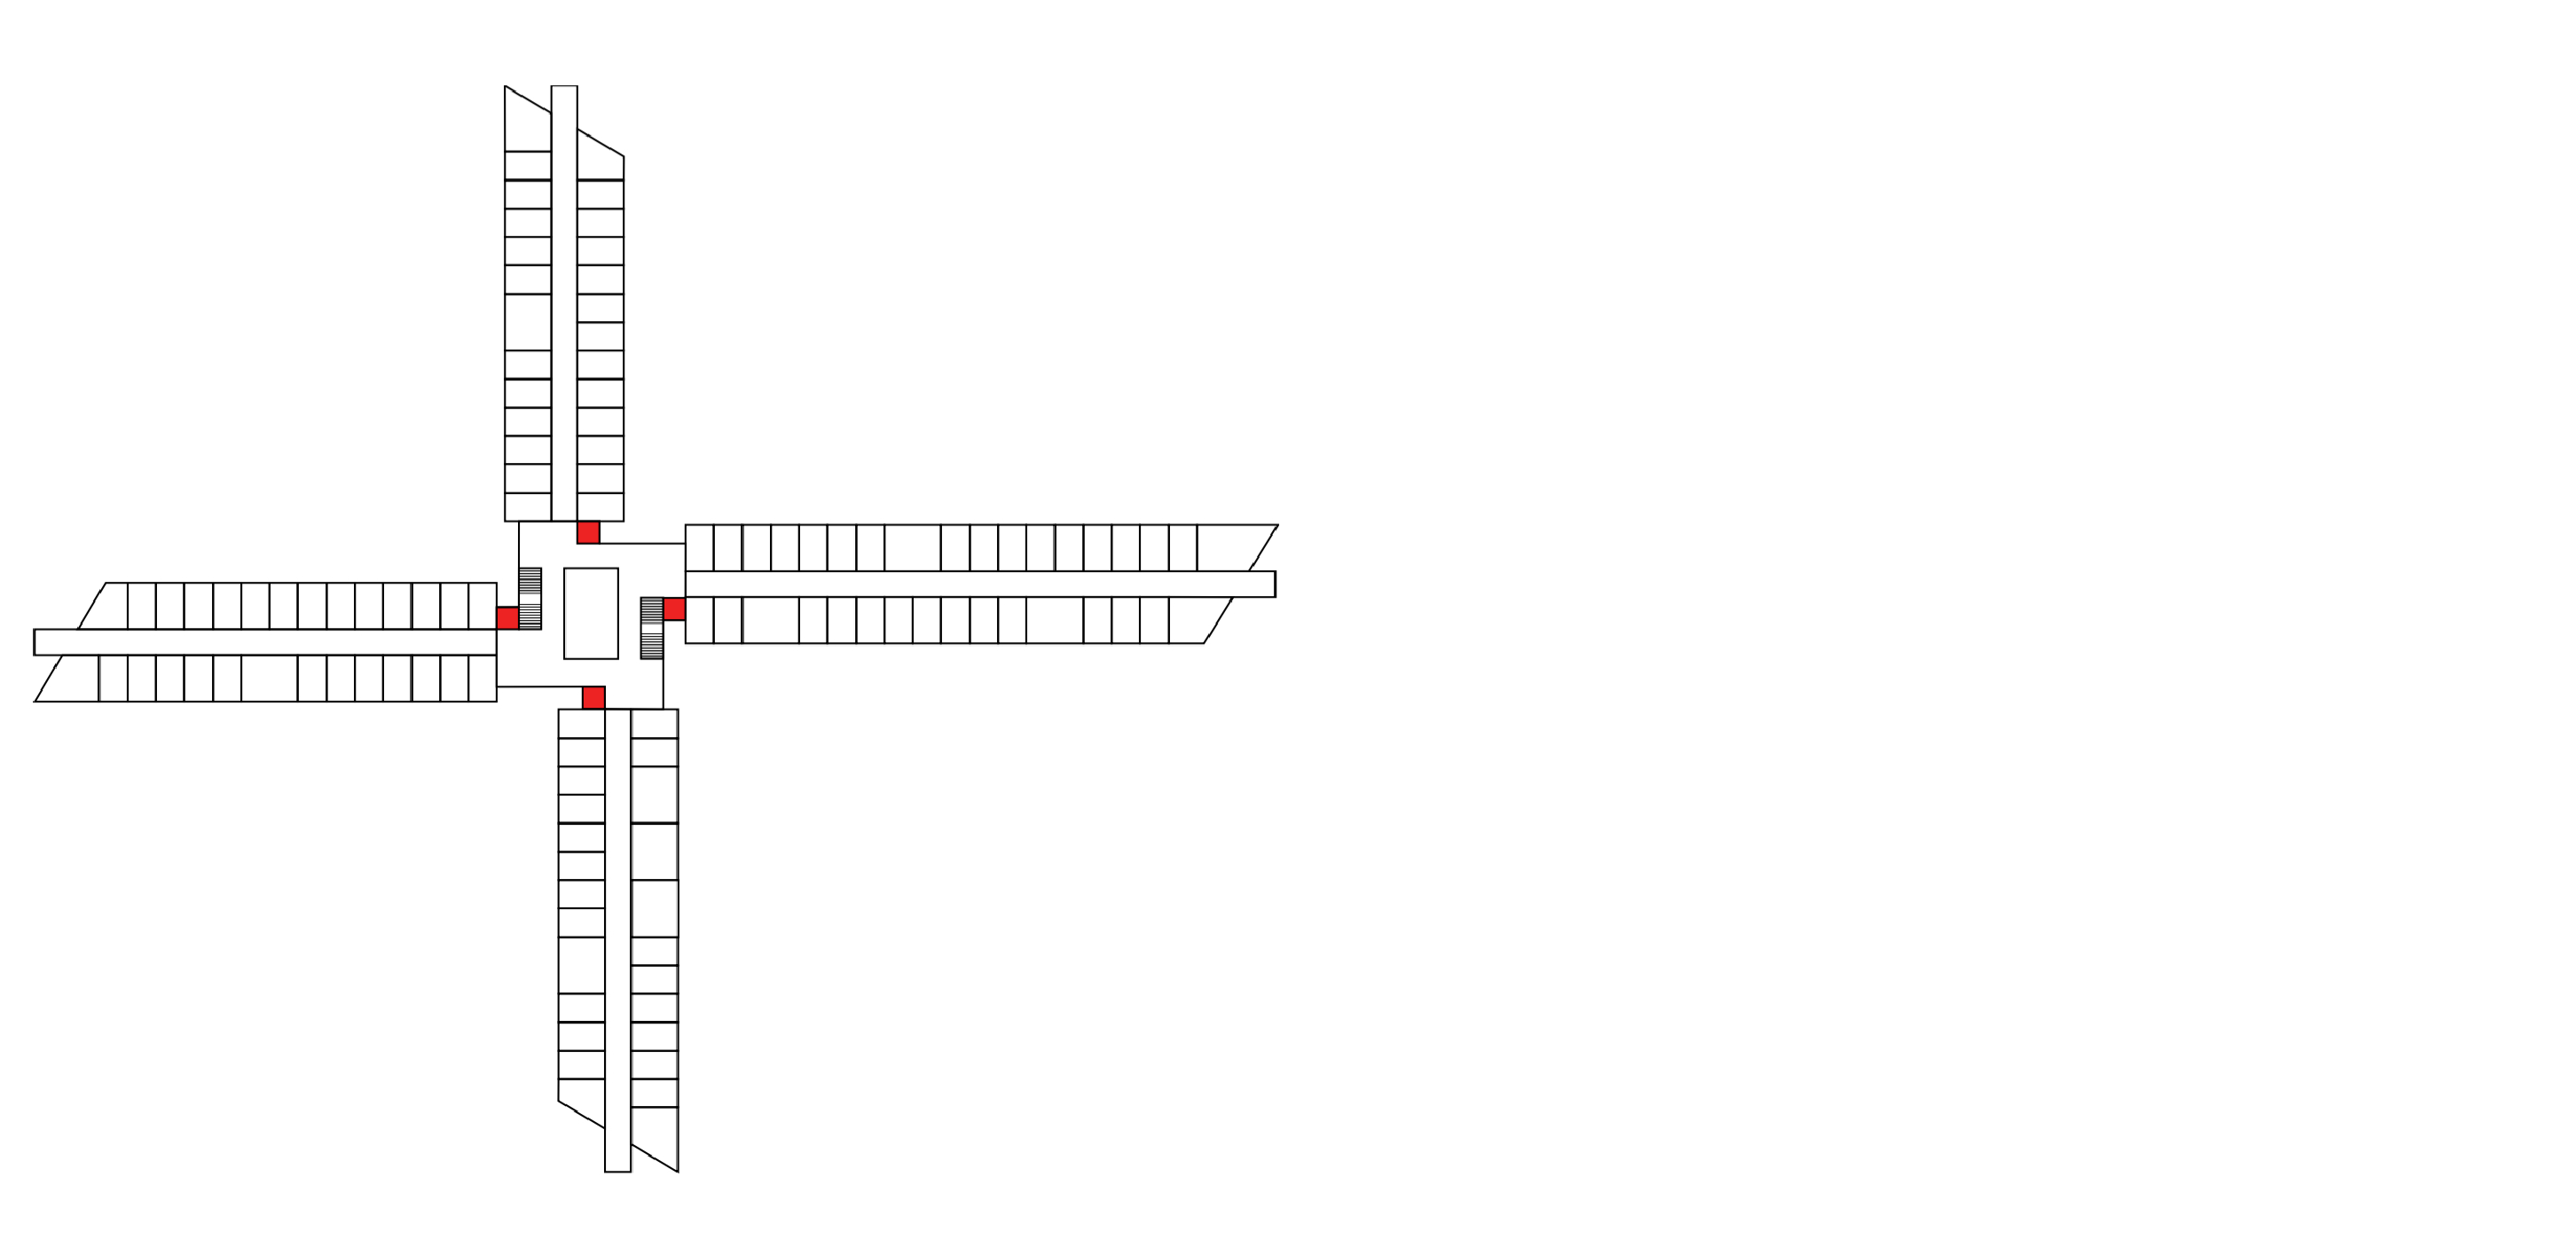
\includegraphics[width=\textwidth]{images/sogei-a} 
 \caption{}
 \label{fig:sogei-a}
 \end{subfigure}
 ~
 \begin{subfigure}[b]{0.48\linewidth}
 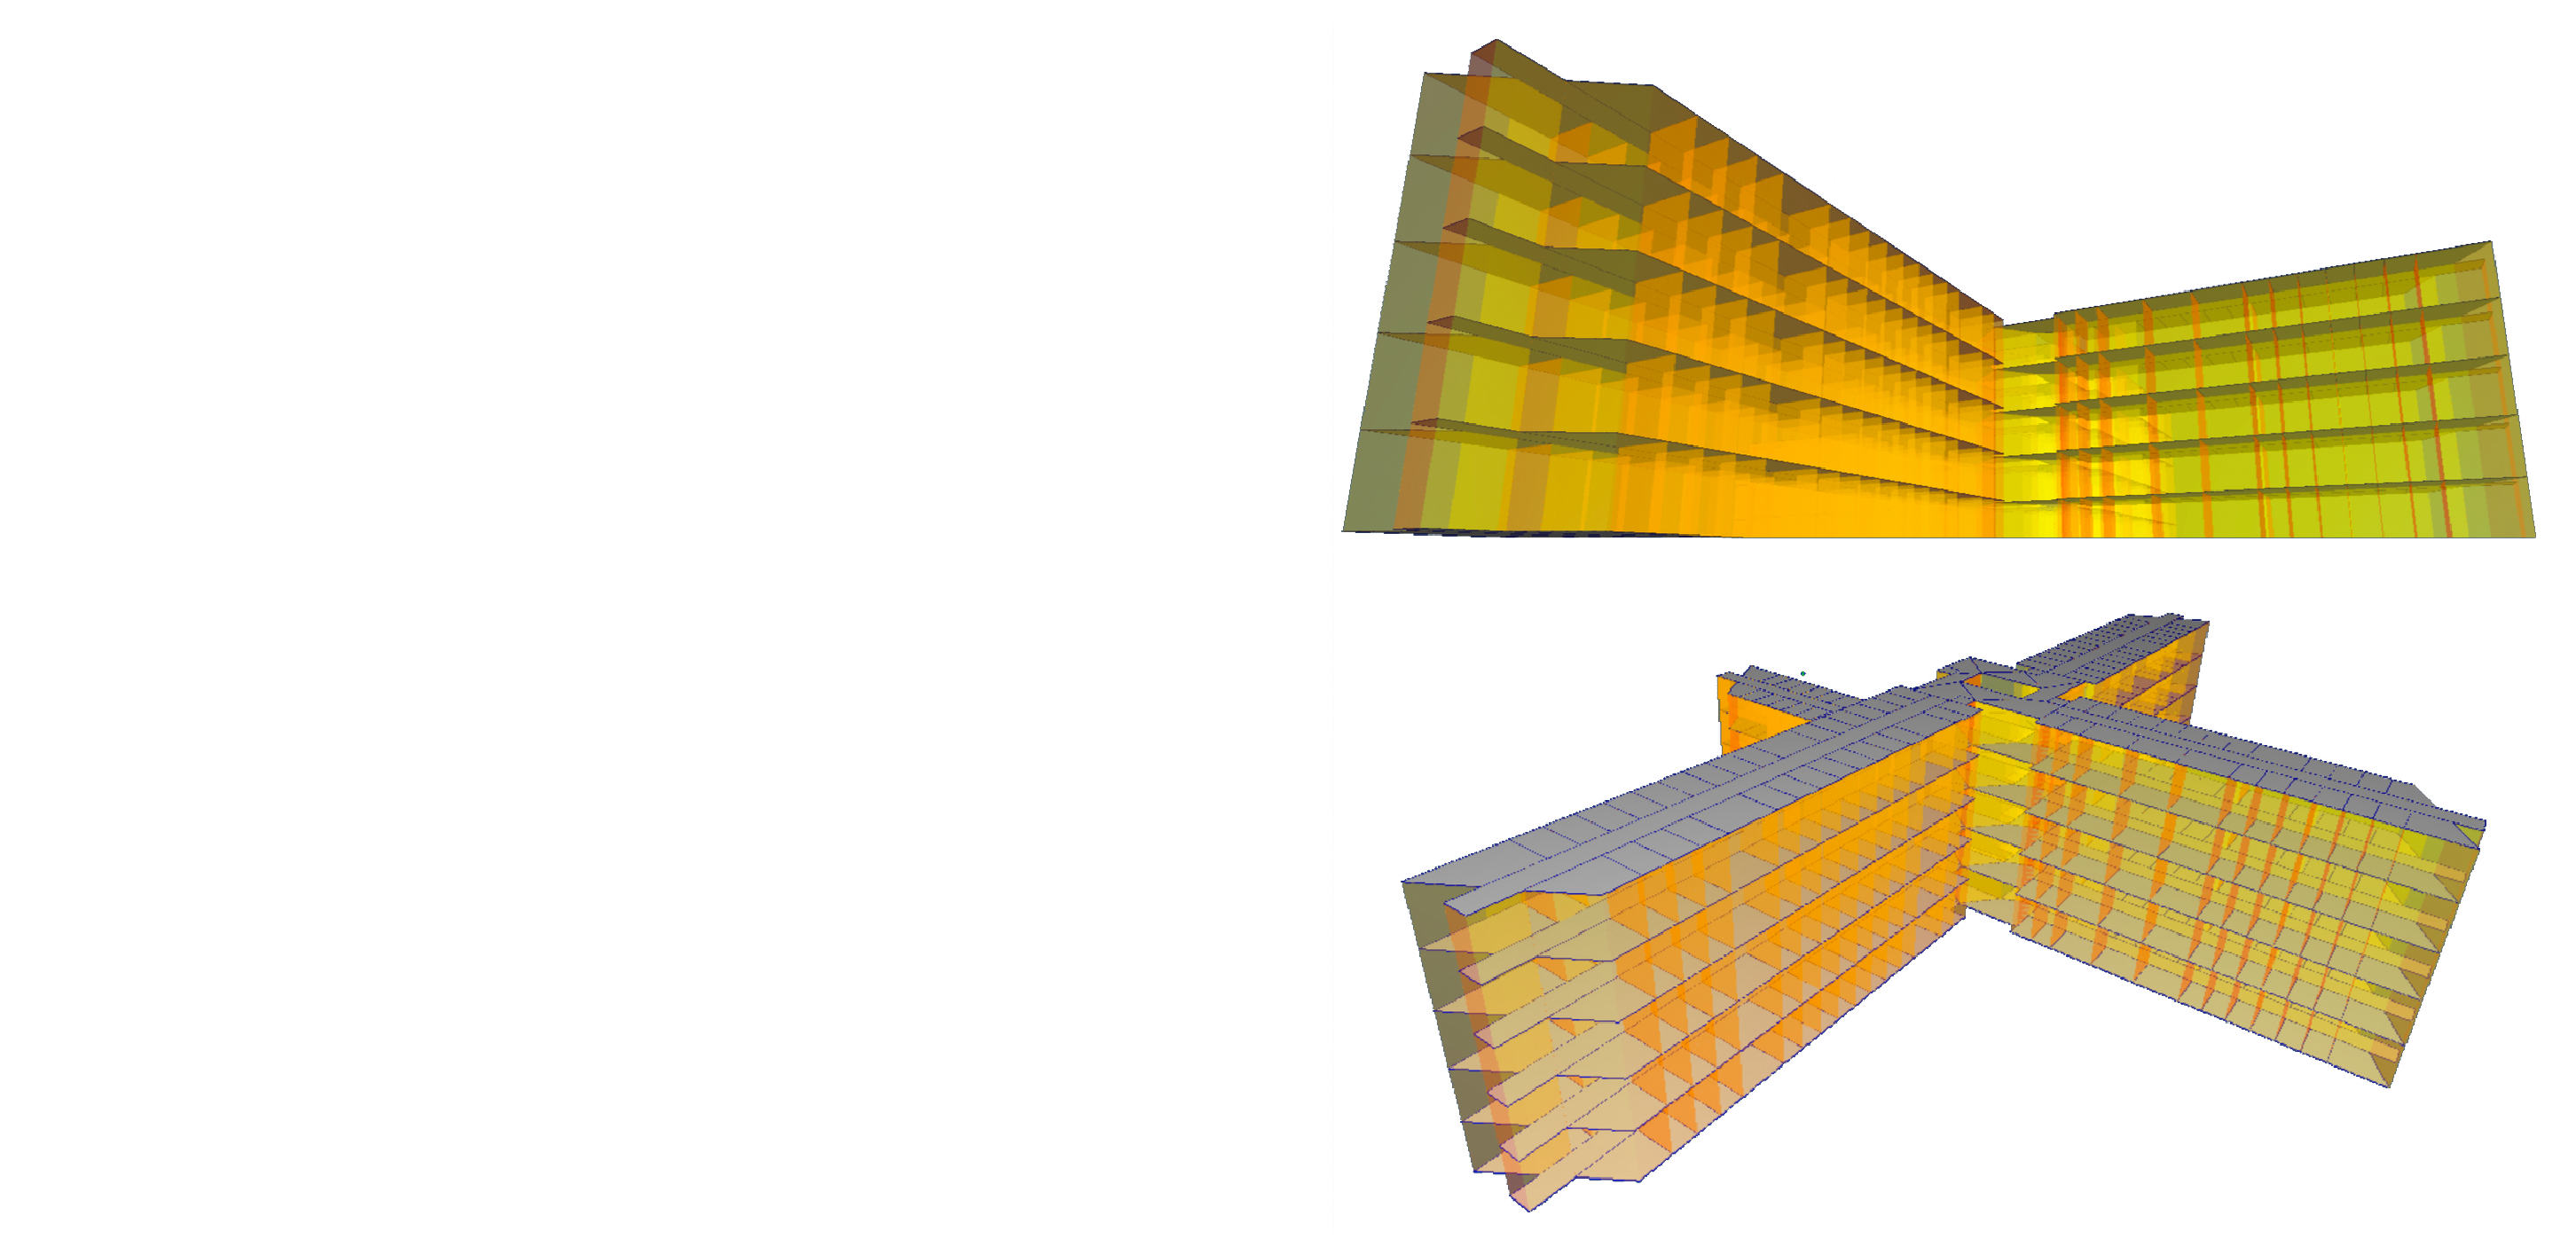
\includegraphics[width=\textwidth]{images/sogei-b}
 \caption{}
 \label{fig:sogei-b}
 \end{subfigure}
 
 \caption{Office building: 
 (a) the schematic plan; 
 (b) the simplified 3D model generated for testing on the field 
 the indoor mapping project described in this paper.
 }
 \label{fig:sogei}
\end{figure}

\subsection{Semantic extensions}\label{semantic-extensions}

Semantic extensions make the HIJSON format extendible and customizable, that
is able to adequately respond to any need of objects representation. To define a
semantic extension means to allow the HIJSON document to model an object
previously not covered, or even to modify the behavior of a comprised one.
Semantic extensions are to be defined both as HIJSON format syntax and as
HIJSON Toolkit source code. In particular it is necessary to define respectively
a new HIJSON Element and a new HIJSON Class, as specified below.

